\documentclass[../main.tex]{subfiles}

\begin{document}
\begin{figure}[H]
\begin{tabular}{c c}
    \begin{subfigure}{0.5\textwidth} 
        \centering
        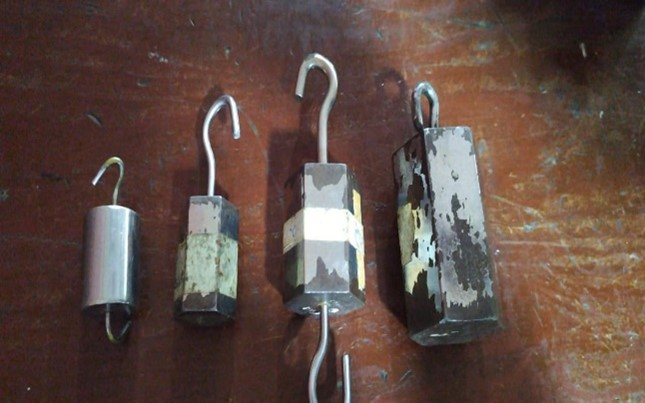
\includegraphics[width=0.8\linewidth,height=0.6\linewidth]{resources/mat1.jpg}
        \caption{Masas}
        \label{fig:mat1}
    \end{subfigure}
    &
    \begin{subfigure}{0.5\textwidth} 
        \centering
        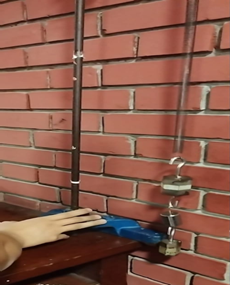
\includegraphics[width=0.8\linewidth,height=0.6\linewidth]{resources/mat2.png}
        \caption{Soporte Universal}
        \label{fig:mat2}
    \end{subfigure}
    \\
    \begin{subfigure}{0.5\textwidth} 
        \centering
        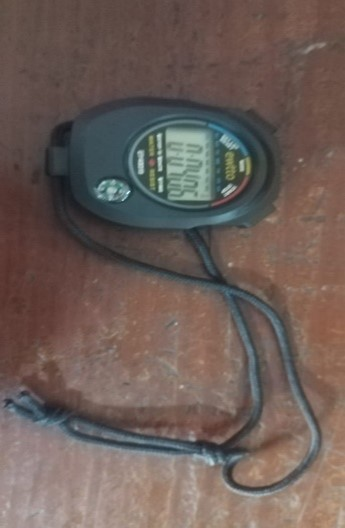
\includegraphics[width=0.8\linewidth,height=0.6\linewidth]{resources/mat3.jpg}
        \caption{Cronómetro}
        \label{fig:mat3}
    \end{subfigure}
    &
    \begin{subfigure}{0.5\textwidth} 
        \centering
        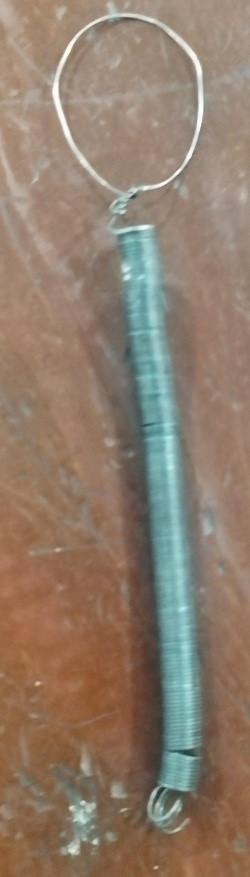
\includegraphics[width=0.8\linewidth,height=0.6\linewidth]{resources/mat4.jpg}
        \caption{Resorte}
        \label{fig:mat4}
    \end{subfigure}
    \\       
    \begin{subfigure}{0.5\textwidth} 
        \centering
        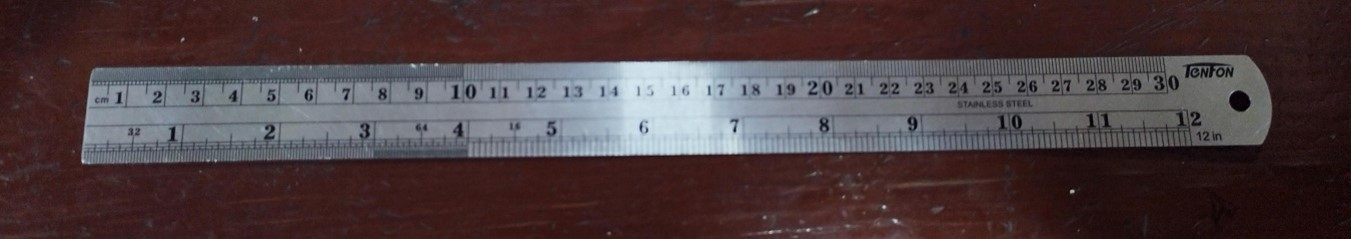
\includegraphics[width=0.8\linewidth,height=0.6\linewidth]{resources/mat5.jpg}
        \caption{Regla}
        \label{fig:mat5}
    \end{subfigure}
    \\
\end{tabular}
\caption{Materiales utilizados.}
\label{fig:mats}
\end{figure}

\end{document}